Ao acessar o sistema através do endereço \textit{https://ipdasuamaquina:40444}, será solicitado um nome de usuário e uma senha para poder entrar no sistema e configurá-lo, como mostra a figura \ref{fig:entrada}.

\begin{figure}[ht]
     \centering
     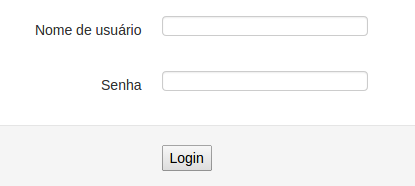
\includegraphics[scale=0.6]{images/entrada.png}
     \caption{Entrada no sistema}
     \label{fig:entrada}
\end{figure}

    Entre com o usuário padrão "administrator" e a senha "icpedu". Será mostrado uma tela para cadastro do novo administrador do sistema, como mostra a figura \ref{fig:inicioadmin}.

\begin{figure}[ht]
     \centering
     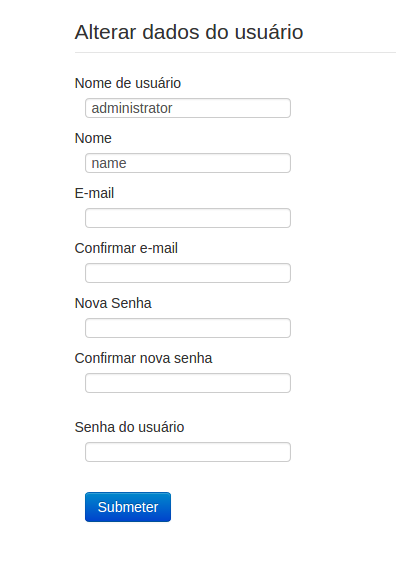
\includegraphics[scale=0.5]{images/inicioadmin.png}
     \caption{Cadastro do administrador}
     \label{fig:inicioadmin}
\end{figure}

    Preencha os campos com a informação exigida, sem deixar nada em branco. 
    
    Grave bem o "Nome de usuário" e a "Nova senha", pois a partir de agora estas serão as credenciais exigidas, tanto nas próximas etapas de configuração, quanto nas próximas vezes que desejar entrar no sistema. Em "senha do usuário", insira a senha do administrador anterior "icpedu" para confirmar a operação. Você será redirecionado para a etapa de backup, como mostra a figura \ref{fig:opcaobackup}.
    
    \begin{figure}[ht]
     \centering
     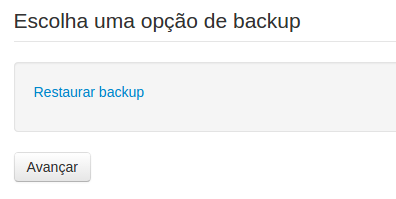
\includegraphics[scale=0.6]{images/opcaobackup.png}
     \caption{Opção de backup}
     \label{fig:opcaobackup}
\end{figure}

    Se existir algum backup do sistema, é possível recuperá-lo nesse passo, clicando em \textit{Restaurar backup} e fazendo upload do arquivo de backup gerado anteriormente. Se não houver backup, ignore esta etapa e clique em \textit{Avançar}. 
    
    Em seguida é necessário escolher uma opção para armazenamento da chave da Autoridade Certificadora. A seguinte tela será mostrada:
    
    \begin{figure}[ht]
     \centering
     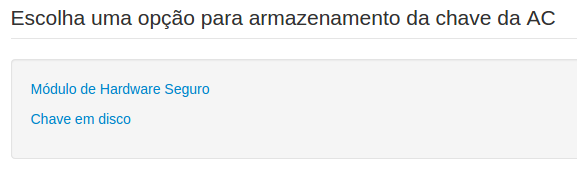
\includegraphics[scale=0.6]{images/armazenachave.png}
     \caption{Opção de armazenamento de chave}
     \label{fig:armazenachave}
\end{figure}

    Se for escolhida a opção "Chave em disco", será solicitada a criação de uma requisição a ser aceita por uma Autoridade Certificadora. Para exemplo, neste manual usaremos a opção "Módulo de Hardware Seguro". Ao optar por esse modo de armazenamento, o usuário será redirecionado para a página de registro e configuração do Módulo de Hardware Seguro, como mostra a figura \ref{fig:confighsm}.
    
    É possível selecionar uma engine já existente no sistema, através da opção \textit{Engine $>$ Selecionar arquivo existente}, ou enviar a sua própria engine, através da opção \textit{Engine $>$ Enviar arquivo}. Independente da escolha, é necessário informar o ID da engine e o identificador da chave do MSC.
    
    Na parte dos comandos, insira o IP e a porta específica de comunicação com o Módulo de Hardware Seguro. Insira sua senha de administrador, escolhida na primeira etapa do cadastro, e clique em \textit{Submeter}.
    
    \begin{figure}[ht]
     \centering
     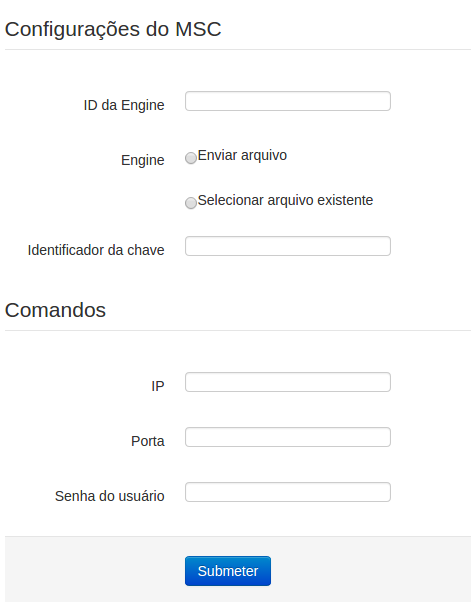
\includegraphics[scale=0.5]{images/confighsm.png}
     \caption{Configuração do MSC}
     \label{fig:confighsm}
\end{figure}

    Depois de configurá-lo, você será redirecionado para a página de criação de requisição para o seu sistema de emissão de certificados ICPEdu. Esta requisição deve ser aprovada por uma Autoridade Certificadora superior, que irá gerar um certificado para o sistema. 

    Preencha os campos da requisição com os dados solicitados sobre sua organização e clique em \textit{Submeter}. Você será redirecionado para a seguinte tela:
    
    \begin{figure}[ht]
     \centering
     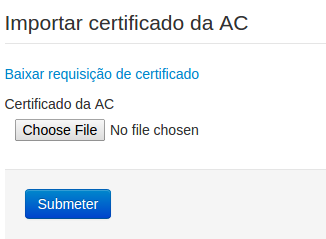
\includegraphics[scale=0.6]{images/importacertAC.png}
     \caption{Importação de certificado}
     \label{fig:reqcert}
\end{figure}

    Baixe a requisição gerada e a envie para uma Autoridade Certificadora, solicitando que esta seja aprovada. Quando isto ocorrer, um certificado será gerado. Faça o download do certificado do seu sistema e importe ele, como mostra a figura \ref{fig:reqcert}.
    
    Em seguida você será redirecionado para a seguinte tela:
    
    \begin{figure}[ht]
     \centering
     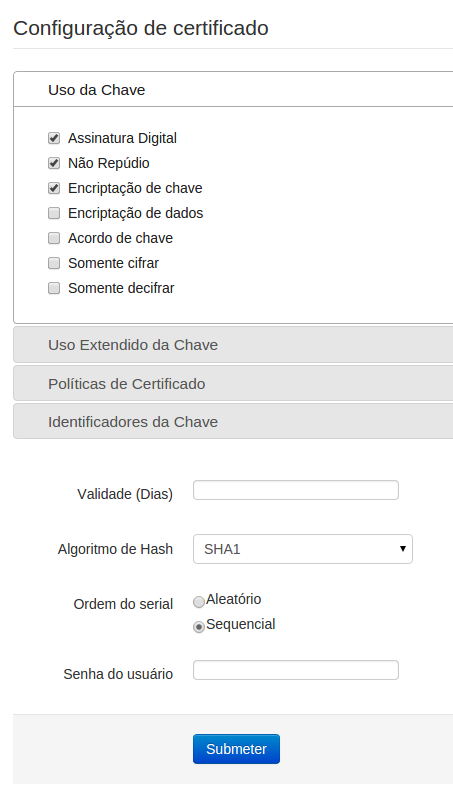
\includegraphics[scale=0.5]{images/configcertificado.png}
     \caption{Configuração do certificado}
     \label{fig:configcertificado}
\end{figure}

    Nesta etapa é possível configurar seu certificado. Algumas opções são definidas por padrão, mas você pode mudá-las se assim desejar. O mesmo serve para o algoritmo de hash e a ordem do serial do certificado. É obrigatório fornecer a validade do seu certificado em dias. Por fim, insira sua senha de administrador e clique em \textit{Submeter}.
    
    Ao fazer isso, você será redirecionado para a página de configuração de whitelist. Whitelist é uma lista com os IPs das máquinas que estão autorizadas a emitir certificado. Quem gerencia esta lista para cada organização são os respectivos operadores das mesmas. O administrador pode escolher se deseja ou não trabalhar com o sistema de whitelist. Faça sua escolha e clique em \textit{Submeter}.
    
    A próxima etapa da configuração é selecionar a federação a qual o seu sistema pertence. É possível selecionar a Comunidade Acadêmica Federada (CAFe) ou a Chimarrão. Pode-se ainda escolher outra federação não listada, e neste caso deve-se fornecer as URLs da mesma.
    
    Depois de selecionar a federação, você será redirecionado para a última etapa da configuração, que é destinada ao registro do primeiro operador do sistema, como é mostrado na figura a seguir:
    
    \begin{figure}[ht]
     \centering
     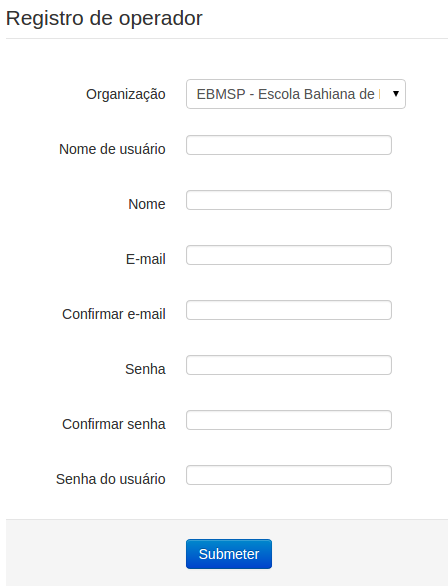
\includegraphics[scale=0.5]{images/inicioregistroop.png}
     \caption{Registro de operador}
     \label{fig:inicioregop}
\end{figure}

    Preencha os dados do operador conforme são solicitados e clique em \textit{Submeter}. Ao fazer isto, a configuração será concluída e você será redirecionado para a página inicial do sistema de emissão de certificados ICPEdu, onde verá o menu funcional do sistema (a ser explicado nos próximos capítulos) e as tarefas pendentes, como mostra a figura a seguir:
    
    \begin{figure}[ht]
     \centering
     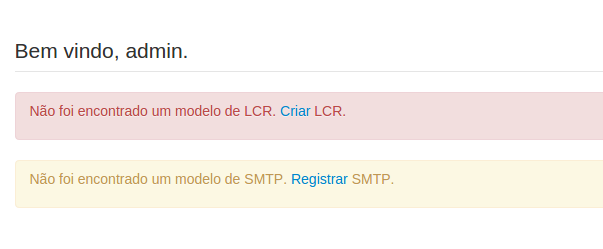
\includegraphics[scale=0.5]{images/pendencias.png}
     \caption{Tarefas pendentes}
     \label{fig:pendencias}
\end{figure}